\section{Durchführung}
\label{sec:Durchführung}
Zu Beginn des Versuchs wird die Filterkurve des Selektivverstärkers untersucht.
Dazu wird an diesen ein Sinusspannungsgenerator angeschlossen. Die Ausgangsspannung
des Verstärkers wird wiederum mit einem Millivoltmeter abgegriffen. Nun wird unter
Variation der Frequenz der Sinusspannung (Amplitude bleibt gleich) die Ausgangsspannung
am Selektivverstärker gemessen und die entsprechenden Werte notiert.

\begin{figure}[H]
  \centering
  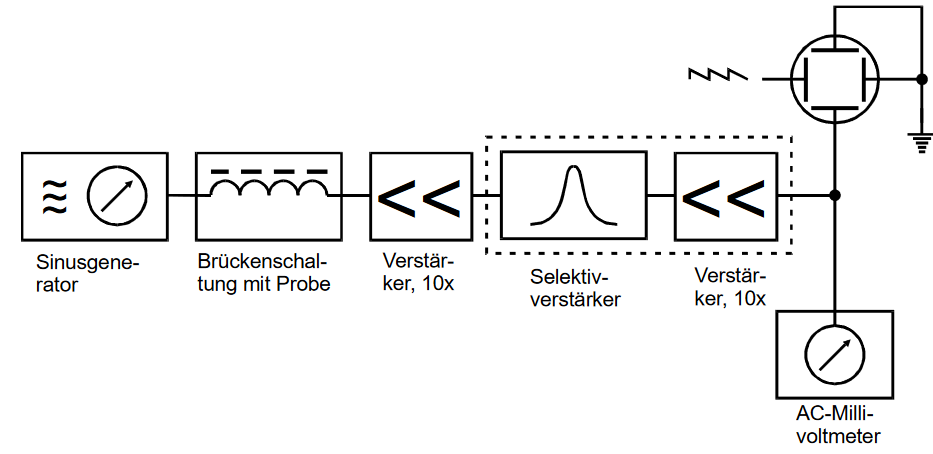
\includegraphics[height=8cm]{Schaltung.PNG}
  \caption{Schaltung der verwendeten Messapparatur. \cite{sample}}
  \label{fig:Schaltung}
\end{figure}

Anschließend wird der Selektivverstärker entsprechend Abbildung \ref{fig:Schaltung}
an eine Brückenschaltung (Abbildung \ref{fig:bruecke}) angeschlossen. Mit einem
Spannungsgenerator wird wieder eine Sinusspannung auf die Brückenschaltung gegeben.
In dieser Konfiguration wird nun das Abgleichpotentiometer so eingestellt, dass an
dem Millivoltmeter ein Minimum der Ausgangsspannung zu erkennen ist. Die entsprechende
Ausgangsspannung und die Einstellung des Potentiometers werden notiert. Im Folgenden werden dann nacheinander die Proben in
die Spule geschoben. Dabei wird die sich dabei ändernde Ausgangsspannung gemessen.
Zudem wird bei jeder Probe das Potentiometer wieder so eingestellt, dass sich ein
Minimum der Spannung ergibt. Auch hier wird wieder dessen Einstellung notiert.
